Исследуется задача о движении волн на поверхности безграничной идеальной несжимаемой жидкости, которая находится в однородном поле сил тяжести. Течение является потенциальным, т.е. для вектора скорости $\vec{u}=\{u,v,w\}$ существует $\phi(x,y,z,t):\vec{u}=grad \phi$. Введём прямоугольную декартову систему координат так, что ось $Oz$ направлена вертикально вверх, в сторону, противоположную направлению ускорения свободного падения, а оси $Ox$ и $Oy$ лежат на невозмущённой свободной поверхности (рис.\;\ref{figure:schema}). Жидкость заполняет область $Q$, ограниченную сверху свободной поверхностью $z=\eta(x,y,t)$, снизу — дном $z=-\tilde{H}(x,y,t)=-H(x,y)+B(x,y,t)$. Здесь $H$ определяет неподвижную часть дна, а $B$ - его динамическую составляющую.

\begin{figure}[htp]
    \centering
    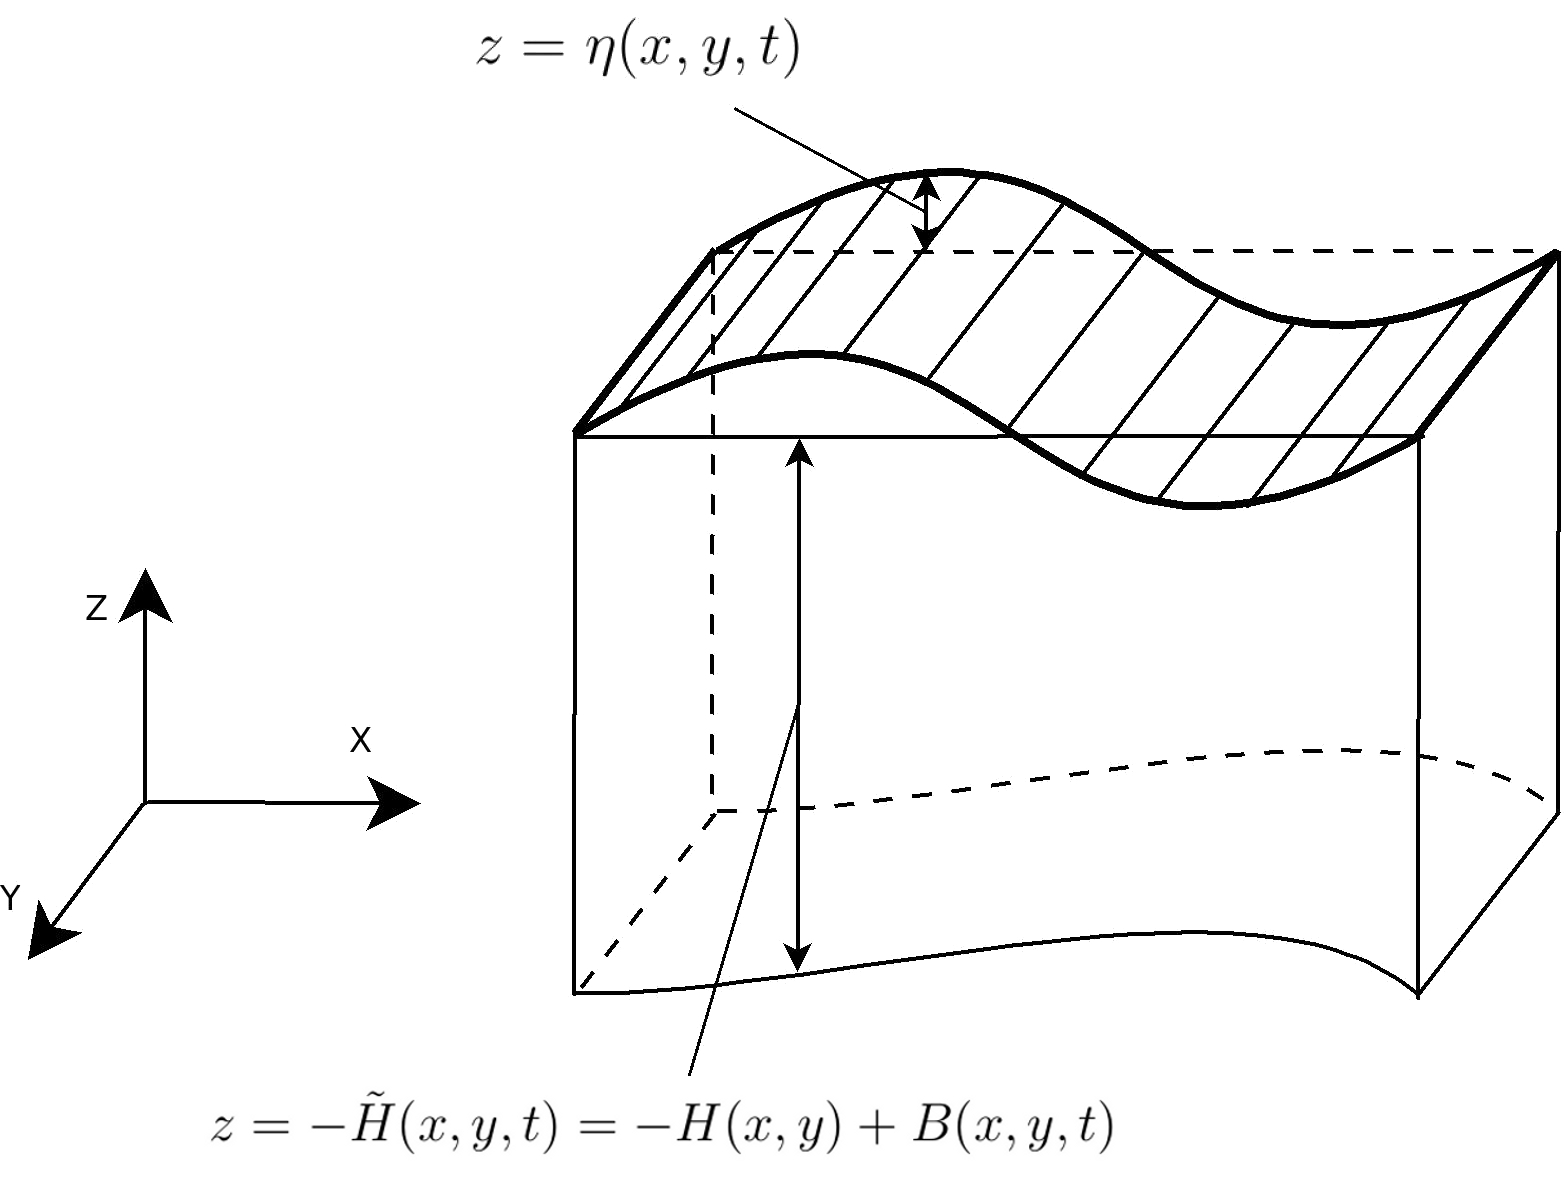
\includegraphics[width=9cm,height=6cm]{scheme.jpg}
    \caption{Постановка задачи}
    \label{figure:schema}
\end{figure}

В качестве физической модели, описывающей данную задачу, взяты уравнения теории мелкой воды (в линейной форме известные также как уравнения Сен-Венана), для которых существенными являются предположения о малости вертикального ускорения частиц жидкости по отношению к ускорению свободного падения и о слабой зависимости горизонтальных скоростей от вертикальной координаты.

Ситуации, когда глубина акватории много меньше горизонтальных размеров, достаточно обычна, поэтому уравнения мелкой воды находят широкое применение. Часто они используются с учётом кориолисовых сил при моделировании атмосферы и океана как упрощение системы примитивных уравнений, описывающих потоки в атмосфере.

Представим уравнения мелкой воды в следующей форме:
\begin{gather}
    \label{eq:MainVectorForm}
    \frac{\partial U}{\partial t}+F_{lin}+F_{nonlin}=\frac{\partial B}{\partial t}\\
    \label{eq:UB}
    U=\begin{pmatrix}\eta\\u\\v\end{pmatrix}
    B=\begin{pmatrix}B(x,y,t)\\0\\0\end{pmatrix}\notag
\end{gather}

\begin{gather}
    \label{eq:FLin}
    F_{lin}=\begin{pmatrix}
	\frac{\partial ((H-B)u)}{\partial x}+\frac{\partial ((H-B)v)}{\partial y}\\
	g\frac{\partial \eta}{\partial x}\\
	g\frac{\partial \eta}{\partial y}
    \end{pmatrix}\\
    \label{eq:FNonLin}
    F_{nonlin}=\begin{pmatrix}
	0\\
	\frac{1}{2}\frac{\partial (u^2)}{\partial x} + v\frac{\partial u}{\partial y}\\
	\frac{1}{2}\frac{\partial (v^2)}{\partial y} + u\frac{\partial v}{\partial x}
    \end{pmatrix}
\end{gather}

%Boundary
\begin{gather}
    \begin{split}
	\label{eq:BoundaryCondition}
	(x,y)&\in\Omega,t>0\\
	u_0=u(x,y,0)\;v_0=&v(x,y,0)\;\eta_0=\eta(x,y,0)\\
	u(x,y,t),v(x,y,t),\eta(&x,y,t)\to0\; x^2+y^2\to\infty
    \end{split}
\end{gather}

	Где $H$ определяет неподвижную часть дна, а $B$ - его динамическую составляющую ($H-B$ – полная грубина слоя жидкости), $\eta$ – функция свободной поверхности, $u(x,y,t)$ – скорость по Ox, $v(x,y,t)$ - скорость по Oy, $g=9,8$. 

	Данные формулы являются гиперболической системой дифференциальных уравнений и описывают более общую постановку задачи в нелинейном виде без учёта сил Кориолиса, трения и вязкости в бесконечной области (более подробно об уравнениях мелкой воды см. \cite{ovsjannikov},\cite{marchyk}). Линейная форма может быть получена как частный случай - для этого достаточно отбросить $F_{nonlin}$.